Verrano descritti di seguito i casi d'uso individuati per il progetto \PROGETTO. Ogni caso d'uso ha un codice che lo indentifica nella forma:
\begin{center}
	UC[codice univoco del padre].[codice progressivo di livello]
\end{center}
Il codice progressivo di livello potrà contenere diversi altri livelli di gerarchia, essi saranno separati da un punto. Per comodità e chiarezza lo scenario principale verrà individuato attraverso il codice UCP. Successivamente verranno descritti i figli senza però riportare il codice del padre.

\subsection{Caso d'uso UCP: Scenario principale}
\begin{figure}[h] 
	\centering 
	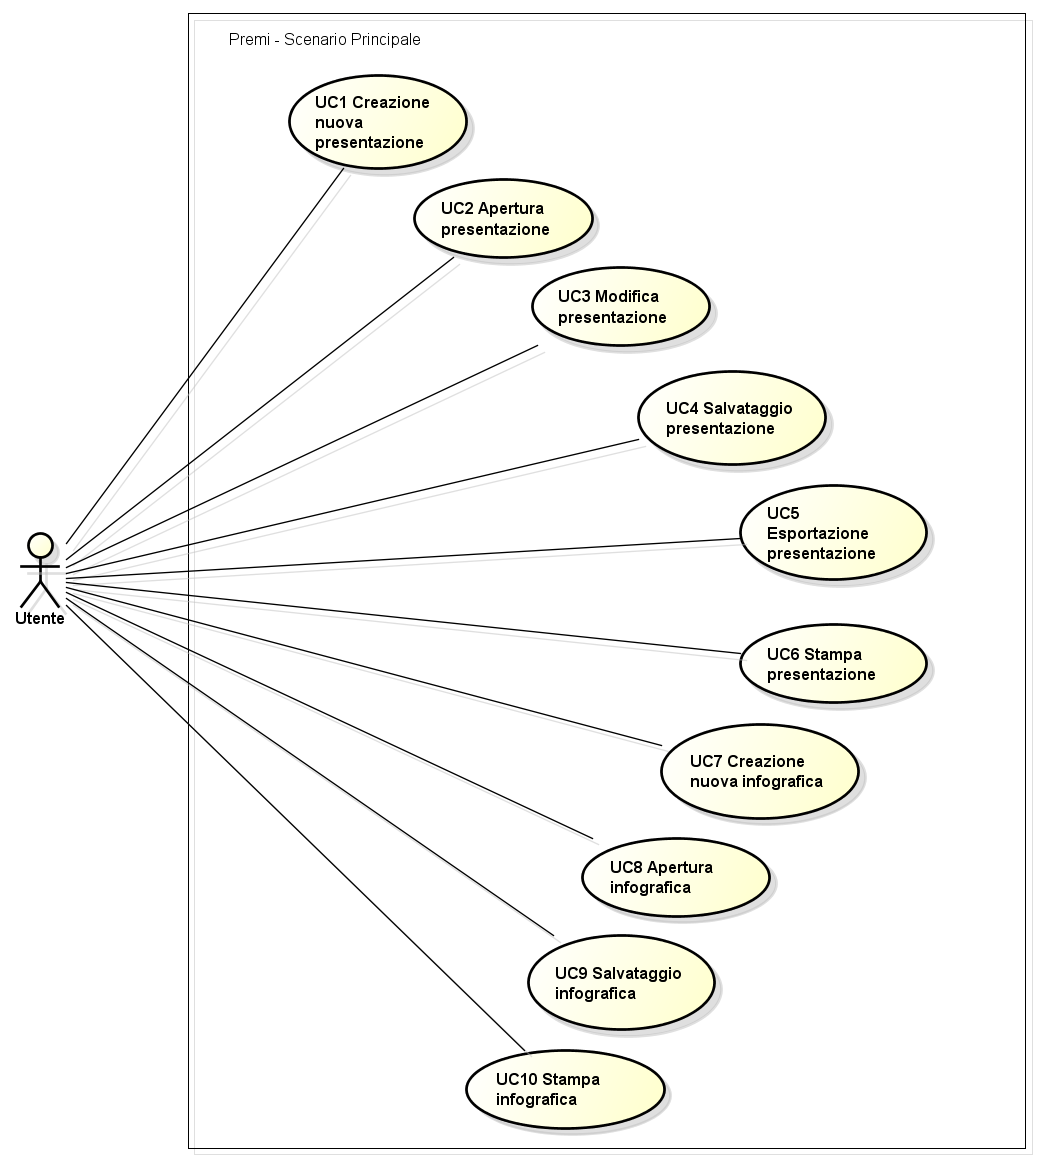
\includegraphics[scale=0.5] {img/UCP.png} 
	\caption{UCP - Scenario principale} 
\end{figure}

\newpage

\begin{itemize}
	\item \textbf{Attori:} Utente;
	\item \textbf{Scopo e descrizione:} Dopo aver avviato il programma, l'utente potrà effettuare diverse operazioni. Potrà creare una nuova presentazione o caricarne una precedentemente creata. Analogamente potrà creare una nuova infografica oppure caricarne una già creata. Se è aperta una presentazione o una infografica l'utente potrà modificare e salvare i nuovi cambiamenti o esportare l'intera presentazione (o infografica). Inoltre l'utente avrà a disposizione una funzione di stampa per stampare le slide della presentazione oppure l'infografica;
	\item \textbf{Precondizione:} Il programma è stato correttamente avviato ed è pronto all'uso;
	\item \textbf{Flusso degli eventi:}
	\begin{enumerate}
		\item L'utente può creare una nuova presentazione [UC1];
		\item L'utente può aprire una presentazione [UC2];
		\item L'utente può modificare una presentazione [UC3];
		\item L'utente può salvare una presentazione [UC4];
		\item L'utente può esportare una presentazione [UC5];
		\item L'utente può stampare una presentazione [UC6];
		\item L'utente può creare una nuova infografica [UC7];
		\item L'utente può aprire una infografica [UC8];
		\item L'utente può salvare una infografica [UC9];
		\item L'utente può stampare una infografica [UC10].
	\end{enumerate}
	\item \textbf{Postcondizione:} Il sistema ha ottenuto le informazioni sulle operazioni che l’utente desidera eseguire.
\end{itemize}

\newpage
\subsection{Caso d'uso UC1: Registrazione}
\begin{figure}[h] 
	\centering 
	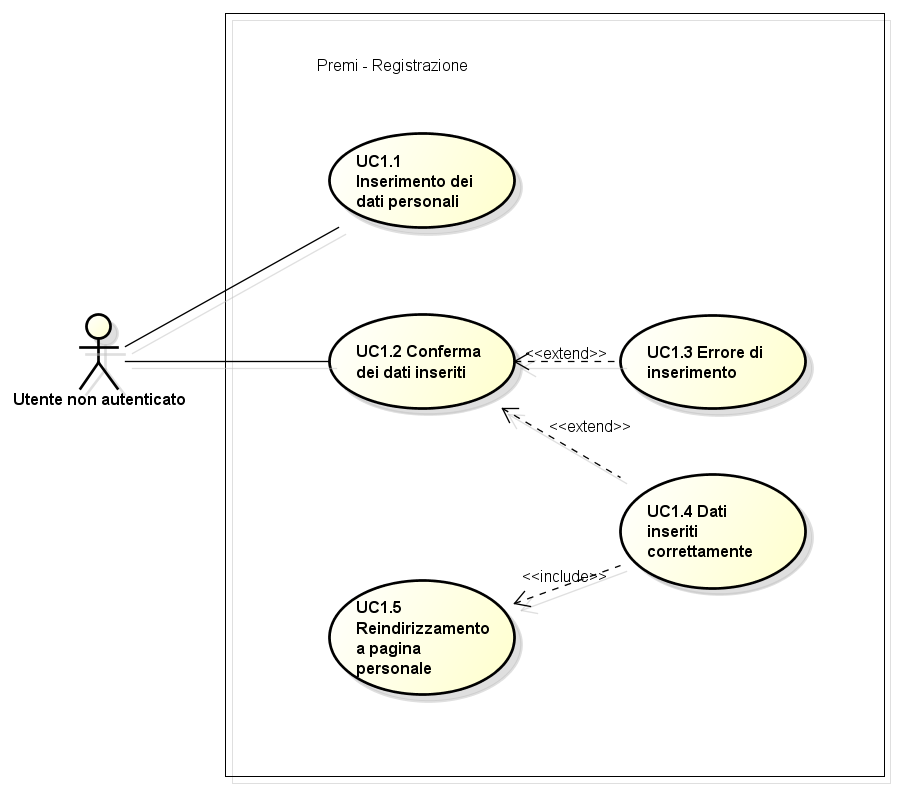
\includegraphics[scale=0.45] {img/UC1.png} 
	\caption{UC1 - Registrazione} 
\end{figure}

\begin{itemize}
	\item \textbf{Attori:} Utente non autenticato;
	\item \textbf{Scopo e descrizione:} L'utente non è iscritto e vuole avviare la procedura di iscrizione al sito;
	\item \textbf{Precondizione:} L'utente ha selezionato la voce "registrati" presente sul sito;
	\item \textbf{Flusso principale degli eventi:}
	\begin{enumerate}
		\item L'utente inserisce i propri dati personali [UC1.1];
		\item L'utente conferma l'inserimento dei propri dati [UC1.2];
		\item Si può verificare un errore di inserimento [UC1.3];
		\item I dati sono stati inseriti correttamente [UC1.4];
		\item Il sistema reindirizza l'utente alla sua pagina personale [UC1.5];
	\end{enumerate}
	\item \textbf{Postcondizione:} Il sistema ha registrato il nuovo utente e lo ha reindirizzato alla propria pagina personale.
\end{itemize}

\newpage

\subsection{Caso d'uso UC1.1: Inserimento dati personali}
\begin{figure}[h] 
	\centering 
	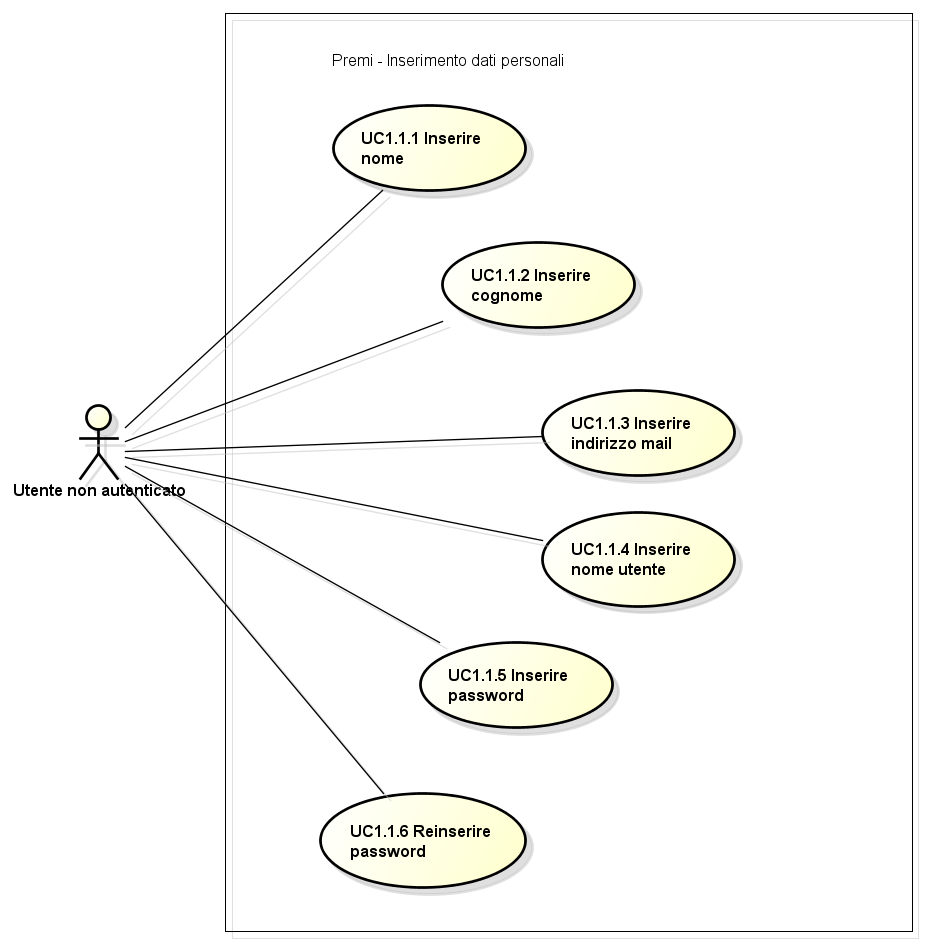
\includegraphics[scale=0.45] {img/UC1.1.png} 
	\caption{UC1.1 - Inserimento dati personali} 
\end{figure}
\begin{itemize}
	\item \textbf{Attori:} Utente non autenticato;
	\item \textbf{Scopo e descrizione:} L'utente inserisce tutti i dati richiesti per la registrazione;
	\item \textbf{Precondizione:} L'utente visualizza la schermata di inserimento dei dati richiesti per la registrazione;
	\item \textbf{Flusso principale degli eventi:}
	\begin{enumerate}
		\item L'utente inserisce il proprio nome [UC1.1.1];
		\item L'utente inserisce il proprio cognome [UC1.1.2];
		\item L'utente inserisce il proprio indirizzo mail [UC1.1.3];
		\item L'utente inserisce il proprio nome utente [UC1.1.4];
		\item L'utente inserisce una password [UC1.1.5];
		\item L'utente inserisce nuovamente la password [UC1.1.6].
	\end{enumerate}
	\item \textbf{Postcondizione:} Tutti i campi richiesti sono stati compilati correttamente.
\end{itemize}

\subsection{Caso d'uso UC1.1.1: Inserire nome}
\begin{itemize}
	\item \textbf{Attori:} Utente non autenticato;
	\item \textbf{Scopo e descrizione:} L'utente inserisce il proprio nome;
	\item \textbf{Precondizione:} La casella dove inserire il nome è vuota;
	\item \textbf{Postcondizione:} La casella è stata compilata con il nome inserito dall'utente.
\end{itemize}

\subsection{Caso d'uso UC1.1.2: Inserire cognome}
\begin{itemize}
	\item \textbf{Attori:} Utente non autenticato;
	\item \textbf{Scopo e descrizione:} L'utente inserisce il proprio cognome;
	\item \textbf{Precondizione:} La casella dove inserire il cognome è vuota;
	\item \textbf{Postcondizione:} La casella è stata compilata con il cognome inserito dall'utente.
\end{itemize}

\subsection{Caso d'uso UC1.1.3: Inserire indirizzo mail}
\begin{itemize}
	\item \textbf{Attori:} Utente non autenticato;
	\item \textbf{Scopo e descrizione:} L'utente inserisce il proprio indirizzo mail;
	\item \textbf{Precondizione:} La casella dove inserire l'indirizzo mail è vuota;
	\item \textbf{Postcondizione:} La casella è stata compilata con l'indirizzo mail inserito dall'utente.
\end{itemize}

\subsection{Caso d'uso UC1.1.4: Inserire nome utente}
\begin{itemize}
	\item \textbf{Attori:} Utente non autenticato;
	\item \textbf{Scopo e descrizione:} L'utente inserisce il proprio nome utente;
	\item \textbf{Precondizione:} La casella dove inserire il nome utente è vuota;
	\item \textbf{Postcondizione:} La casella è stata compilata con il nome utente inserito dall'utente.
\end{itemize}

\subsection{Caso d'uso UC1.1.5: Inserire password}
\begin{itemize}
	\item \textbf{Attori:} Utente non autenticato;
	\item \textbf{Scopo e descrizione:} L'utente inserisce la propria password;
	\item \textbf{Precondizione:} La casella dove inserire la password è vuota;
	\item \textbf{Postcondizione:} La casella è stata compilata con la password inserita dall'utente.
\end{itemize}

\subsection{Caso d'uso UC1.1.6: Reinserire password}
\begin{itemize}
	\item \textbf{Attori:} Utente non autenticato;
	\item \textbf{Scopo e descrizione:} L'utente inserisce nuovamente la password inserita in precedenza;
	\item \textbf{Precondizione:} La casella dove inserire la password è già stata compilata e la casella dove reinserire per la seconda volta la password è vuota;
	\item \textbf{Postcondizione:} La casella di reinserimento password è stata compilata con la password inserita dall'utente.
\end{itemize}

\subsection{Caso d'uso UC1.2: Conferma dei dati inseriti}
\begin{itemize}
	\item \textbf{Attori:} Utente non autenticato;
	\item \textbf{Scopo e descrizione:} L'utente deve confermare i dati inseriti in precedenza per procedere con l'iscrizione;
	\item \textbf{Precondizione:} L'utente ha inserito i dati richiesti per la registrazione;
	\item \textbf{Postcondizione:} Il sistema elabora i dati e registra il nuovo utente.
\end{itemize}

\subsection{Caso d'uso UC1.3: Errore di inserimento}
\begin{itemize}
	\item \textbf{Attori:} Sistema;
	\item \textbf{Scopo e descrizione:} Dopo che l'utente ha confermato i dati, il sistema segnala all'utente che c'è stato un errore di inserimento e mostra nuovamente la schermata di inserimento dei dati personali;
	\item \textbf{Precondizione:} L'utente ha confermato i dati inseriti;
	\item \textbf{Postcondizione:} Il sistema segnala all'utente che c'è stato un errore di inserimento e mostra di nuovo la schermata di inserimento dei dati personali.
\end{itemize}

\subsection{Caso d'uso UC1.4: Dati inseriti correttamente}
\begin{itemize}
	\item \textbf{Attori:} Sistema;
	\item \textbf{Scopo e descrizione:} Dopo che l'utente ha confermato i dati inseriti, il sistema li controlla e li accetta;
	\item \textbf{Precondizione:} L'utente ha confermato i dati inseriti;
	\item \textbf{Postcondizione:} Il sistema controlla e accetta i dati inseriti dall'utente.
\end{itemize}

\subsection{Caso d'uso UC1.5: Reindirizzamento a pagina personale}
\begin{itemize}
	\item \textbf{Attori:} Sistema;
	\item \textbf{Scopo e descrizione:} Dopo aver confermato i propri dati, il sistema reindirizza l'utente alla propria pagina personale dove può accedere alle varie funzionalità del sito;
	\item \textbf{Precondizione:} Il sistema ha registrato correttamente il nuovo utente;
	\item \textbf{Postcondizione:} Il sistema permette all'utente di visualizzare la propria pagina personale.
\end{itemize}

\subsection{Caso d'uso UC2: Autenticazione}
\begin{figure}[h] 
	\centering 
	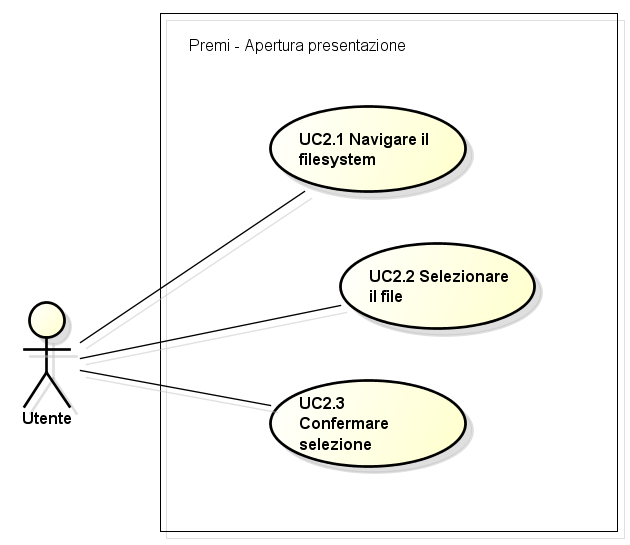
\includegraphics[scale=0.45] {img/UC2.png}
	\caption{UC2 - Autenticazione} 
\end{figure}

\begin{itemize}
	\item \textbf{Attori:} Utente non autenticato;
	\item \textbf{Scopo e descrizione:} L'utente è già iscritto e vuole avviare la procedura di autenticazione al sito per accedere ai propri file;
	\item \textbf{Precondizione:} L'utente ha selezionato la voce "accedi" presente sul sito;
	\item \textbf{Flusso principale degli eventi:}
	\begin{enumerate}
		\item L'utente inserisce le proprie credenziali [UC2.1];
		\item L'utente conferma l'inserimento dei dati selezionando la voce "login" [UC2.2];
		\item Si può verificare un errore di accesso [UC2.3];
		\item Il sistema controlla i dati inseriti e li accetta [UC2.4];
		\item L'utente viene reindirizzato alla propria pagina personale [UC2.5];
		\item L'utente può recuperare le sue credenziali se le dimentica [UC2.6].
	\end{enumerate}
	\item \textbf{Postcondizione:} Il sistema verifica le credenziali inserite e permette all'utente di accedere alla sua pagina personale.
\end{itemize}

\subsection{Caso d'uso UC2.1: Inserimento credenziali}
\begin{figure}[h] 
	\centering 
	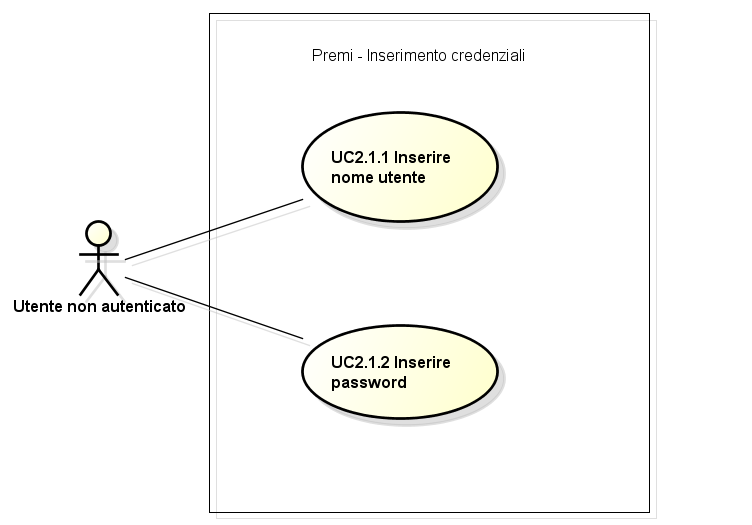
\includegraphics[scale=0.45] {img/UC2.1.png}
	\caption{UC2.1 - Inserimento credenziali} 
\end{figure}
\begin{itemize}
	\item \textbf{Attori:} Utente non autenticato;
	\item \textbf{Scopo e descrizione:} L'utente inserisce nome utente e password per poter accedere al sito;
	\item \textbf{Precondizione:} L'utente visualizza la schermata di inserimento dei dati richiesti per l'accesso;
	\item \textbf{Flusso principale degli eventi:}
	\begin{enumerate}
		\item L'utente inserisce il proprio nome utente [UC2.1.1];
		\item L'utente inserisce la propria password [UC2.1.2];
	\end{enumerate}
	\item \textbf{Postcondizione:} Tutti i campi richiesti sono stati compilati correttamente.
\end{itemize}

\subsection{Caso d'uso UC2.1.1: Inserire nome utente}
\begin{itemize}
	\item \textbf{Attori:} Utente non autenticato;
	\item \textbf{Scopo e descrizione:} L'utente inserisce il proprio nome utente;
	\item \textbf{Precondizione:} La casella dove inserire il nome utente è vuota;
	\item \textbf{Postcondizione:} La casella è stata compilata con il nome utente inserito dall'utente.
\end{itemize}

\subsection{Caso d'uso UC2.1.2: Inserire password}
\begin{itemize}
	\item \textbf{Attori:} Utente non autenticato;
	\item \textbf{Scopo e descrizione:} L'utente inserisce la propria password;
	\item \textbf{Precondizione:} La casella dove inserire la password è vuota;
	\item \textbf{Postcondizione:} La casella è stata compilata con la password inserita dall'utente.
\end{itemize}

\subsection{Caso d'uso UC2.2: Accesso}
\begin{itemize}
	\item \textbf{Attori:} Utente non autenticato;
	\item \textbf{Scopo e descrizione:} L'utente conferma le credenziali inserite scegliendo di effettuare l'accesso tramite il tasto di login;
	\item \textbf{Precondizione:} Nome utente e password sono stati inseriti;
	\item \textbf{Postcondizione:} Il sistema verifica i dati inseriti.
\end{itemize}

\subsection{Caso d'uso UC2.3: Errore di autenticazione}
\begin{itemize}
	\item \textbf{Attori:} Sistema;
	\item \textbf{Scopo e descrizione:} L'utente ha inserito delle credenziali errate e il sistema blocca l'accesso, riportando l'utente alla schermata di accesso;
	\item \textbf{Precondizione:} Nome utente e password sono stati inseriti in modo errato;
	\item \textbf{Postcondizione:} Il sistema riporta l'utente alla schermata di accesso.
\end{itemize}

\subsection{Caso d'uso UC2.4: Dati inseriti correttamente}
\begin{itemize}
	\item \textbf{Attori:} Sistema;
	\item \textbf{Scopo e descrizione:} Il sistema ha verificato che le credenziali inserite sono corrette;
	\item \textbf{Precondizione:} Nome utente e password sono stati inseriti;
	\item \textbf{Postcondizione:} Il sistema ha verificato che i dati inseriti sono corretti.
\end{itemize}

\subsection{Caso d'uso UC2.5: Reindirizzamento a pagina personale}
\begin{itemize}
	\item \textbf{Attori:} Sistema;
	\item \textbf{Scopo e descrizione:} Il sistema dopo aver consentito l'accesso all'utente mostra la sua pagina personale;
	\item \textbf{Precondizione:} Nome utente e password sono stati inseriti correttamente;
	\item \textbf{Postcondizione:} Il sistema mostra la pagina personale dell'utente.
\end{itemize}

\subsection{Caso d'uso UC2.6: Recupero dati}
\begin{figure}[h] 
	\centering 
	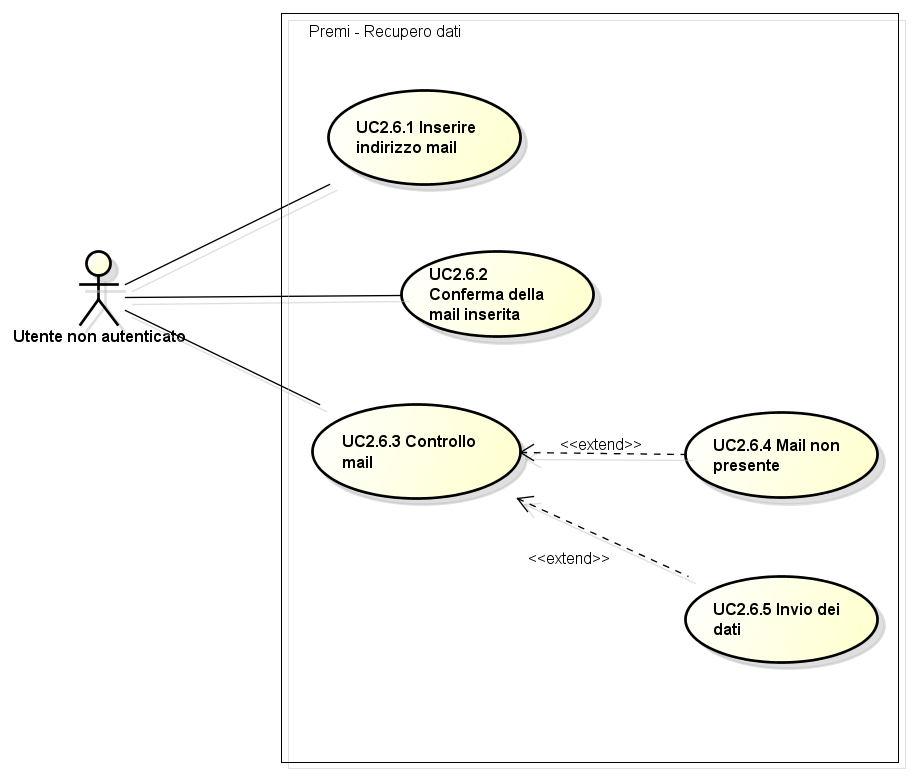
\includegraphics[scale=0.45] {img/UC2.6.png}
	\caption{UC2.6 - Recupero dati} 
\end{figure}
\begin{itemize}
	\item \textbf{Attori:} Utente non autenticato;
	\item \textbf{Scopo e descrizione:} L'utente non ricorda più le sue credenziali di accesso e sceglie quindi l'opzione per il recupero di tali dati. Il sistema gestirà la richiesta inviando all'indirizzo e-mail dell'utente tutti i suoi dati;
	\item \textbf{Precondizione:} L'utente ha selezionato l'opzione di recupero dei dati;
	\item \textbf{Flusso principale degli eventi:}
	\begin{enumerate}
		\item L'utente inserisce il proprio indirizzo mail [UC2.6.1];
		\item L'utente conferma l'inserimento dell'indirizzo mail [UC2.6.2];
		\item Il sistema controlla l'indirizzo e-mail inserita [UC2.6.3];
		\item Il sistema non trova l'indirizzo e-mail nel \gls{database} e segnala un errore [2.6.4];
		\item Il sistema trova una corrispondenza con l'indirizzo e-mail indicato e invia i dati [2.6.5].
	\end{enumerate}
	\item \textbf{Postcondizione:} Il sistema ha inviato una mail contenente i dati di accesso relativi all'utente che ne ha fatto richiesta.
\end{itemize}

\subsection{Caso d'uso UC2.6.1: Inserire indirizzo mail}
\begin{itemize}
	\item \textbf{Attori:} Utente non autenticato;
	\item \textbf{Scopo e descrizione:} L'utente inserisce il proprio indirizzo e-mail nella casella vuota;
	\item \textbf{Precondizione:} La casella dove inserire l'indirizzo e-mail è vuota;
	\item \textbf{Postcondizione:} La casella è stata compilata con l'indirizzo e-mail inserito dall'utente.
\end{itemize}

\subsection{Caso d'uso UC2.6.2: Conferma della mail inserita}
\begin{itemize}
	\item \textbf{Attori:} Utente non autenticato;
	\item \textbf{Scopo e descrizione:} L'utente conferma la mail inserita in precedenza e invia la richiesta;
	\item \textbf{Precondizione:} L'utente ha inserito un indirizzo e-mail;
	\item \textbf{Postcondizione:} L'utente ha confermato l'indirizzo e-mail inserito.
\end{itemize}

\subsection{Caso d'uso UC2.6.3: Controllo mail}
\begin{itemize}
	\item \textbf{Attori:} Sistema;
	\item \textbf{Scopo e descrizione:} Il sistema controlla che l'e-mail inserita dall'utente sia già presente nel \gls{database};
	\item \textbf{Precondizione:} L'utente ha confermato l'inserimento del proprio indirizzo e-mail;
	\item \textbf{Postcondizione:} Il sistema ha controllato che l'indirizzo e-mail inserito esista nel \gls{database}.
\end{itemize}

\subsection{Caso d'uso UC2.6.4: Indirizzo e-mail non presente}
\begin{itemize}
	\item \textbf{Attori:} Sistema;
	\item \textbf{Scopo e descrizione:} Il sistema non trova l'indirizzo e-mail nel \gls{database} e lo segnala all'utente;
	\item \textbf{Precondizione:} Il sistema ha controllato l'indirizzo e-mail inserito e non ha trovato corrispondenze nel \gls{database};
	\item \textbf{Postcondizione:} Il sistema avvisa l'utente che l'e-mail inserita non esiste nel \gls{database}.
\end{itemize}

\subsection{Caso d'uso UC2.6.5: Invio dei dati}
\begin{itemize}
	\item \textbf{Attori:} Sistema;
	\item \textbf{Scopo e descrizione:} Il sistema ha trovato l'indirizzo e-mail nel \gls{database} e invia le credenziali alla mail dell'utente;
	\item \textbf{Precondizione:} Il sistema ha controllato l'indirizzo e-mail inserito e ha trovato una corrispondenza nel \gls{database};
	\item \textbf{Postcondizione:} Il sistema invia le credenziali all'indirizzo e-mail indicata all'utente e avvisa l'utente dell'avvenuto invio.
\end{itemize}



\subsection{Caso d'uso UC3: Ricerca di un progetto}
\begin{figure}[h] 
	\centering 
	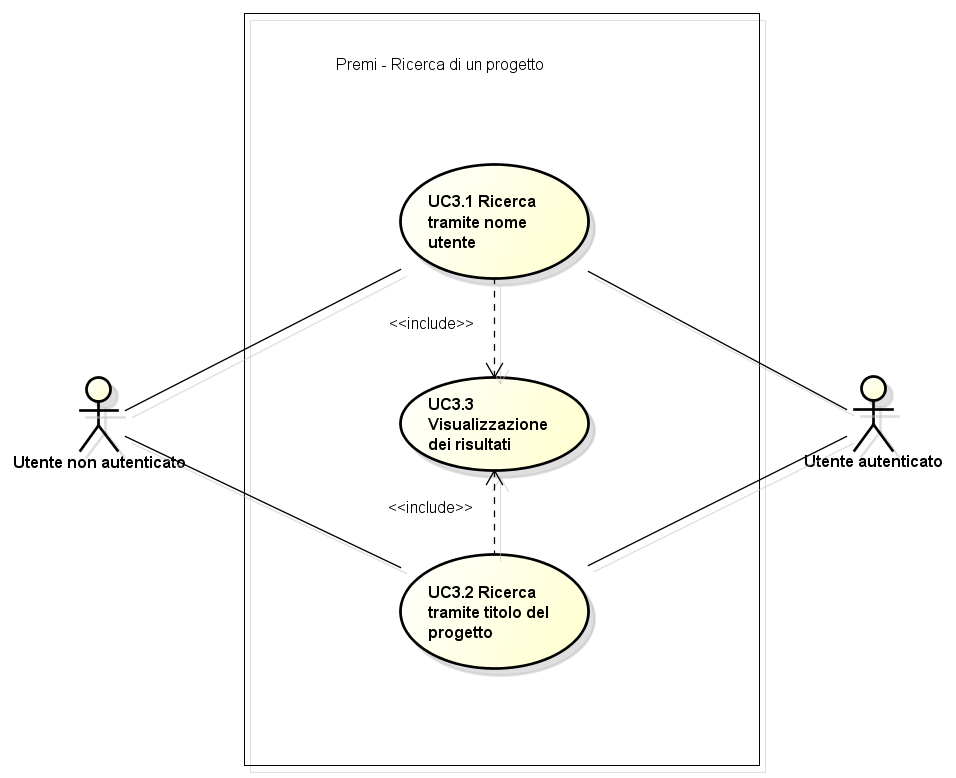
\includegraphics[scale=0.45] {img/UC3.png} 
	\caption{UC3 - Ricerca di un progetto} 
\end{figure}

\begin{itemize}
	\item \textbf{Attori:} Utente non autenticato, utente autenticato;
	\item \textbf{Scopo e descrizione:} L'utente può cercare un progetto utilizzando come chiave di ricerca il nome utente o il titolo del progetto;
	\item \textbf{Precondizione:} L'utente sta visualizzando la schermata di ricerca;
	\item \textbf{Flusso principale degli eventi:}
	\begin{enumerate}
		\item Ricerca tramite nome utente [UC3.1]
		\item Ricerca tramite titolo del progetto [UC3.2]
	\end{enumerate}
	\item \textbf{Postcondizione:} Il sistema mostra all'utente il risultato della ricerca visualizzando l'anteprima, il titolo e l'autore per ogni progetto.
\end{itemize}

\subsection{Caso d'uso UC3.1: Ricerca tramite nome utente}
\begin{itemize}
	\item \textbf{Attori:} Utente non autenticato, utente autenticato;
	\item \textbf{Scopo e descrizione:} L'utente inserisce nella casella di ricerca il nome utente di un creatore di un progetto;
	\item \textbf{Precondizione:} L'utente sta visualizzando la schermata di ricerca. Estende il caso d'uso UC3;
	\item \textbf{Postcondizione:} L'utente ha inserito un nome utente nella casella di ricerca ed ha avviato la ricerca.
\end{itemize}

\subsection{Caso d'uso UC3.2: Ricerca tramite titolo del progetto}
\begin{itemize}
	\item \textbf{Attori:} Utente non autenticato, utente autenticato;
	\item \textbf{Scopo e descrizione:} L'utente inserisce nella casella di ricerca il titolo di un progetto;
	\item \textbf{Precondizione:} L'utente sta visualizzando la schermata di ricerca. Estende il caso d'uso UC3;
	\item \textbf{Postcondizione:} L'utente ha inserito un titolo nella casella di ricerca ed ha avviato la ricerca.
\end{itemize}


\subsection{Caso d'uso UC4: Visualizzazione}
\begin{figure}[h] 
	\centering 
	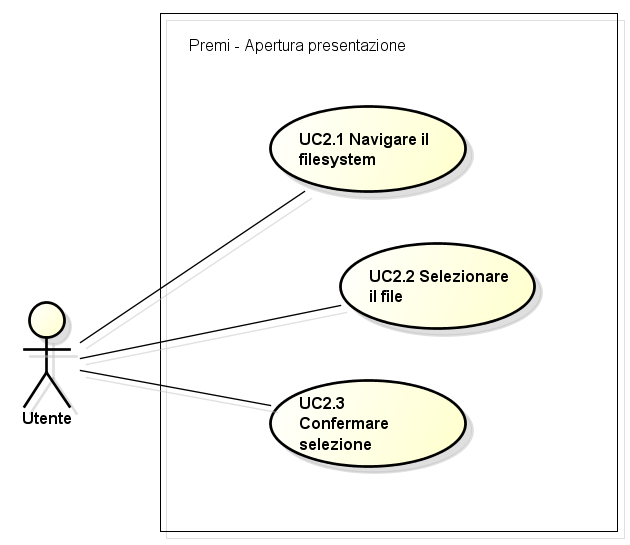
\includegraphics[scale=0.45] {img/UC4.png}
	\caption{UC4 - Visualizzazione} 
\end{figure}

\begin{itemize}
	\item \textbf{Attori:} Utente non autenticato, utente autenticato;
	\item \textbf{Scopo e descrizione:} Un utente, una volta aperto un progetto, può scegliere se visualizzare una presentazione o un'\gls{infografica};
	\item \textbf{Precondizione:} Il sistema mostra all'utente un progetto;
	\item \textbf{Flusso principale degli eventi:}
	\begin{enumerate}
		\item L'utente sceglie di visualizzare una presentazione [UC4.1];
		\item L'utente sceglie di visualizzare un'\gls{infografica} [UC4.2].
	\end{enumerate}
	\item \textbf{Postcondizione:} Il sistema mostra all'utente la schermata di visualizzazione di una presentazione o di un'\gls{infografica} a seconda di cosa è stato scelto.
\end{itemize}

\subsection{Caso d'uso UC4.1: Visualizzazione di una presentazione}
\begin{figure}[h] 
	\centering 
	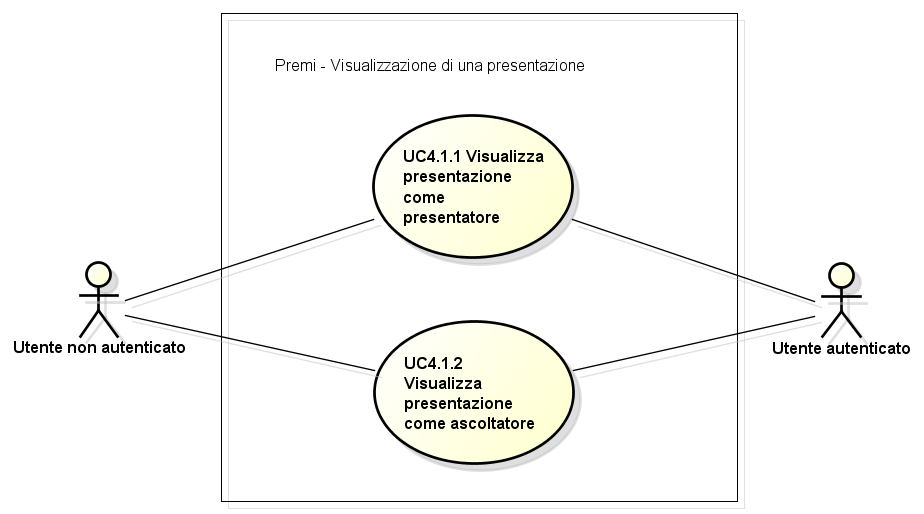
\includegraphics[scale=0.45] {img/UC4.1.png}
	\caption{UC4.1 - Visualizzazione di una presentazione} 
\end{figure}

\begin{itemize}
	\item \textbf{Attori:} Utente non autenticato, utente autenticato;
	\item \textbf{Scopo e descrizione:} La visualizzazione di una presentazione permette di scorrere le \gls{slide} nelle quattro direzioni a seconda di come sono state inserite. In generale, la presentazione segue un flusso principale (da sinistra a destra) nel quale sono presenti i capitoli principali, e un flusso secondario di dettaglio (dall'alto verso il basso) per ogni capitolo che si desidera, nel quale si può esplicitare l'argomento trattato.\\
	Durante il passaggio da un capitolo all'altro avverrà un effetto di "zoom-out, zoom-in" con il quale è possibile avere una panoramica della presentazione e soprattutto delle \gls{slide} del capitolo che si andrà ad affrontare.\\
	Una volta scelto di visualizzare una presentazione, l'utente può scegliere se visualizzarla come presentatore o come ascoltatore;
	\item \textbf{Precondizione:} L'utente ha scelto di visualizzare una presentazione;
	\item \textbf{Flusso principale degli eventi:}
	\begin{enumerate}
		\item L'utente sceglie di visualizzare la presentazione come presentatore [UC4.1.1];
		\item L'utente sceglie di visualizzare la presentazione come ascoltatore [UC4.1.2].
	\end{enumerate}
	\item \textbf{Postcondizione:} Il sistema mostra all'utente la schermata di visualizzazione di una presentazione con le impostazioni scelte.
\end{itemize}

\subsection{Caso d'uso UC4.1.1: Visualizzare una presentazione come presentatore}
\begin{itemize}
	\item \textbf{Attori:} Utente non autenticato, utente autenticato;
	\item \textbf{Scopo e descrizione:} L'utente ha scelto di visualizzare la presentazione come presentatore e il sistema mostra la presentazione con il supporto visivo dedicato al presentatore;
	\item \textbf{Precondizione:} L'utente ha scelto di visualizzare la presentazione come presentatore;
	\item \textbf{Postcondizione:} Il sistema avvia la presentazione con il supporto visivo dedicato al presentatore.
\end{itemize}

\subsection{Caso d'uso UC4.1.2: Visualizzare una presentazione come ascoltatore}
\begin{itemize}
	\item \textbf{Attori:} Utente non autenticato, utente autenticato;
	\item \textbf{Scopo e descrizione:} L'utente ha scelto di visualizzare la presentazione come ascoltatore e il sistema mostra la presentazione selezionata;
	\item \textbf{Precondizione:} L'utente ha scelto di visualizzare la presentazione come ascoltatore;
	\item \textbf{Postcondizione:} Il sistema avvia la presentazione.
\end{itemize}

\subsection{Caso d'uso UC4.2: Visualizzazione di un'infografica}
\begin{itemize}
	\item \textbf{Attori:} Utente non autenticato, utente autenticato;
	\item \textbf{Scopo e descrizione:} L'utente ha scelto di visualizzare un'\gls{infografica} e il sistema la mostra;
	\item \textbf{Precondizione:} L'utente ha scelto di visualizzare un'\gls{infografica};
	\item \textbf{Postcondizione:} Il sistema mostra all'utente la schermata di visualizzazione dell'\gls{infografica}.
\end{itemize}



\subsection{Caso d'uso UC5: Esportazione della presentazione}
	\begin{figure}[h] 
		\centering 
		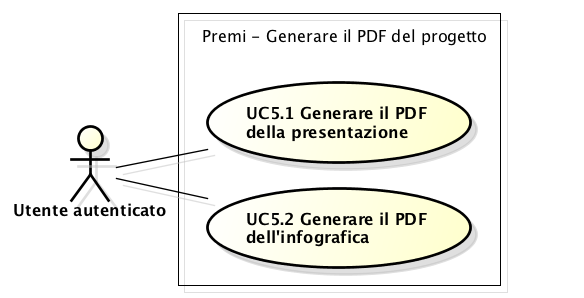
\includegraphics[scale=0.45] {img/UC5.png} 
		\caption{UC5 - Esportazione della presentazione} 
	\end{figure}
	
	\begin{itemize}
		\item \textbf{Attori:} Utente;
		\item \textbf{Scopo e descrizione:} L'utente ha creato una presentazione di slide e vuole esportarla in un formato diverso per salvarla nel proprio computer;
		\item \textbf{Precondizione:} Il sistema è in attesa che l'utente selezione la funzione esporta presentazione;
		\item \textbf{Flusso degli eventi:}
		\begin{enumerate}
			\item L'utente seleziona dal menù la funzione esporta [UC5.1];
			\item L'utente sceglie il formato in cui esportare la presentazione [UC5.2];
			\item L'utente sceglie dove esportare la presentazione [UC5.3];
			\item L'utente conferma l'esportazione [UC5.4];
		\end{enumerate}
		\item \textbf{Postcondizione:} Il sistema ha esportato la presentazione.
	\end{itemize}


\subsection{Caso d'uso UC5.1: Selezionare funzione esporta}
	\begin{itemize}
		\item \textbf{Attori:} Utente;
		\item \textbf{Scopo e descrizione:} L'utente seleziona dal menù la funzione esporta per esportare la presentazione;
		\item \textbf{Precondizione:} Il sistema è in attesa che l'utente selezioni la funzione dal menù;
		\item \textbf{Postcondizione:} Il sistema apre la finestra di dialogo per l'esportazione.
	\end{itemize}


\subsection{Caso d'uso UC5.2: Selezionare il formato di esportazione}
	\begin{itemize}
		\item \textbf{Attori:} Utente;
		\item \textbf{Scopo e descrizione:} L'utente deve scegliere il formato in cui esportare la presentazione;
		\item \textbf{Precondizione:} Il sistema è in attesa che l'utente selezioni il formato dall'apposita finestra di dialogo;
		\item \textbf{Postcondizione:} Il sistema registra la scelta e apre la finestra di dialogo per il salvataggio della presentazione esportata.
	\end{itemize}


\subsection{Caso d'uso UC5.3: Selezionare la destinazione di esportazione}
	\begin{itemize}
		\item \textbf{Attori:} Utente;
		\item \textbf{Scopo e descrizione:} L'utente deve scegliere la destinazione in cui salvare la presentazione esportata.
		\item \textbf{Precondizione:} Il sistema è in attesa che l'utente selezioni il percorso dall'apposita finestra di dialogo;
		\item \textbf{Postcondizione:} Il sistema registra la destinazione desiderata.
	\end{itemize}


\subsection{Caso d'uso UC5.4: Confermare l'esportazione}
	\begin{itemize}
		\item \textbf{Attori:} Utente;
		\item \textbf{Scopo e descrizione:} L'utente deve confermare l'esportazione della presentazione nel formato e nella destinazione desiderata;
		\item \textbf{Precondizione:} Il sistema è in attesa che l'utente confermi l'esportazione;
		\item \textbf{Postcondizione:} Il sistema ha esportato la presentazione.
	\end{itemize}
	
	
\subsection{Caso d'uso UC5.5: Selezionare il percorso}
	\begin{figure}[h] 
		\centering 
		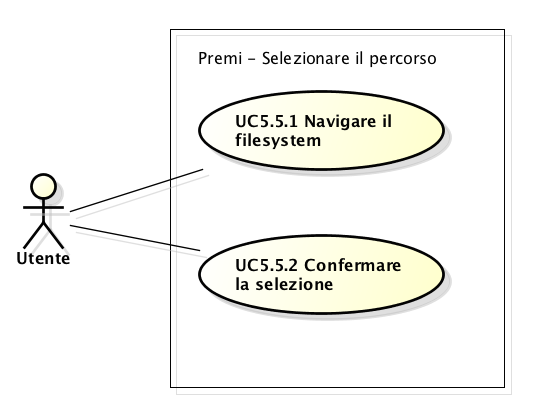
\includegraphics[scale=0.45] {img/UC5.5.png} 
		\caption{UC5.5 - Selezionare il percorso} 
	\end{figure}
	\begin{itemize}
		\item \textbf{Attori:} Utente;
		\item \textbf{Scopo e descrizione:} L'utente deve scegliere il percorso. Naviga il filesystem, lo seleziona ne e conferma la scelta;
		\item \textbf{Precondizione:} Il sistema è in attesa che l'utente navighi il filesystem e confermi il percorso scelto;
		\item \textbf{Flusso degli eventi:}
		\begin{enumerate}
			\item L'utente naviga il filesystem alla ricerca della posizione desiderata [UC5.5.1];
			\item L'utente conferma la posizione selezionata [UC5.5.2].
		\end{enumerate}
		\item \textbf{Postcondizione:} Il sistema registra il percorso desiderato.
	\end{itemize}
	
	\subsection{Caso d'uso UC5.5.1: Navigare il filesystem}
	\begin{itemize}
		\item \textbf{Attori:} Utente;
		\item \textbf{Scopo e descrizione:} L'utente può navigare il filesystem per selezionare la cartella dentro la quale vuole esportare la presentazione;
		\item \textbf{Precondizione:} Il sistema è in attesa che l'utente selezioni una cartella;
		\item \textbf{Postcondizione:} Il sistema ha aggiornato la il percorso con quello scelto dall'utente.
	\end{itemize}
	
	\subsection{Caso d'uso UC5.5.2: Confermare selezione}
	\begin{itemize}
		\item \textbf{Attori:} Utente;
		\item \textbf{Scopo e descrizione:} L'utente conferma che il percorso selezionato è quello corretto;
		\item \textbf{Precondizione:} Il sistema ha selezionato il percorso indicato dall'utente;
		\item \textbf{Postcondizione:} Il sistema ha registrato il percorso precedentemente scelto dall'utente.
	\end{itemize}